\documentclass{article} % For LaTeX2e
\usepackage{nips13submit_e,times}
\usepackage{hyperref}
\usepackage{url}
\usepackage{amsmath}
\usepackage{graphicx,float,wrapfig}
\usepackage{caption}
\usepackage{subcaption}
\usepackage{natbib}
\usepackage{bibhacks}
%\documentstyle[nips13submit_09,times,art10]{article} % For LaTeX 2.09


\title{Probabilistic Matrix Factorization}


\author{ 
  Mert Terzihan \\
  Department of Computer Science\\
  Brown University\\
  Providence, RI 02912 \\
  \texttt{mert\_terzihan@brown.edu}
  \And
  Gabriel Barth-Maron \\
  Department of Computer Science \\
  Brown University \\
  Providence, RI 02912 \\
  \texttt{gabriel\_barth-maron@brown.edu}\\
}

% The \author macro works with any number of authors. There are two commands
% used to separate the names and addresses of multiple authors: \And and \AND.
%
% Using \And between authors leaves it to \LaTeX{} to determine where to break
% the lines. Using \AND forces a linebreak at that point. So, if \LaTeX{}
% puts 3 of 4 authors names on the first line, and the last on the second
% line, try using \AND instead of \And before the third author name.

\newcommand{\fix}{\marginpar{FIX}}
\newcommand{\new}{\marginpar{NEW}}

\nipsfinalcopy % Uncomment for camera-ready version

\begin{document}


\maketitle

\section{Description of the Problem}
\label{desc}
Matrix Factorization is a widely used method, especially in collaborative 
filtering and recommendation systems. With the rise of data available to 
researchers and the requirement to present personalized ads or recommendations 
to users led the researchers to further study of this field. As our final 
project, we will be dealing with Probabilistic Matrix Factorization on 
matrices with discrete values. In particular we will apply these methods to analyze the movie-user review data in the MovieLens 100k dataset \cite{movielens100k}.


\section{Discussion of Related Work}
\label{work}
As studied in \cite{lda} and \cite{discrete-pca}, one can observe that LDA is equivalent to factorizing a matrix 
probabistically using a graphical model representation. Instead of dealing with 
a co-occurence matrix, we will try to propose a model and a learning algorithm to 
factorize a matrix where each cell is a rating of an item by a particular user. 
Therefore, in addition to LDA, we would also like to generate ratings that have been 
assigned by users to each item. 

In \cite{Argwal-fDLA} a method based on LDA is proposed to produce personalized recommendations.
However, fLDA takes into account much more information about the user, i.e. age, 
gender, zipcode, etc. We are going to use a simpler model, which relies on
much less personal information. We will be using only the ratings 
that have been given by the users to specific items.

A LDA-based probabilistic matrix factorization models is proposed in
\cite{conf/icdm/ShanB10}, however instead of using discrete distribution
for generating ratings, it has placed a Gaussian distribution over the user's
ratings. In our investigation we hope to relax this assumption and look into
models that are not necessarily Gaussian.

\section{Graphical Model}
\label{graph}
Below is the graphical model and the details about it, where $j \in U$, $i \in M$ 
and $t \in T$, and $U$ is the total number of users, $M$ is the total number of items, 
and $T$ is the number of topics that we would like to extract. 
\begin{align*}
  &\theta_j \sim Dir(\alpha)\\
  &z_{ji} \sim Cat(\theta_j)\\
  &\phi_g \sim Dir(\beta)\\
  &x_{ji} \sim Cat(\phi_{z_{ji}}) \\
  &\kappa_{tj} \sim Dir(\gamma)\\
  &r_{ji} \sim Cat(\kappa_{z_{ji},j})
\end{align*}
\clearpage
\begin{figure}[h]
    \begin{center}
      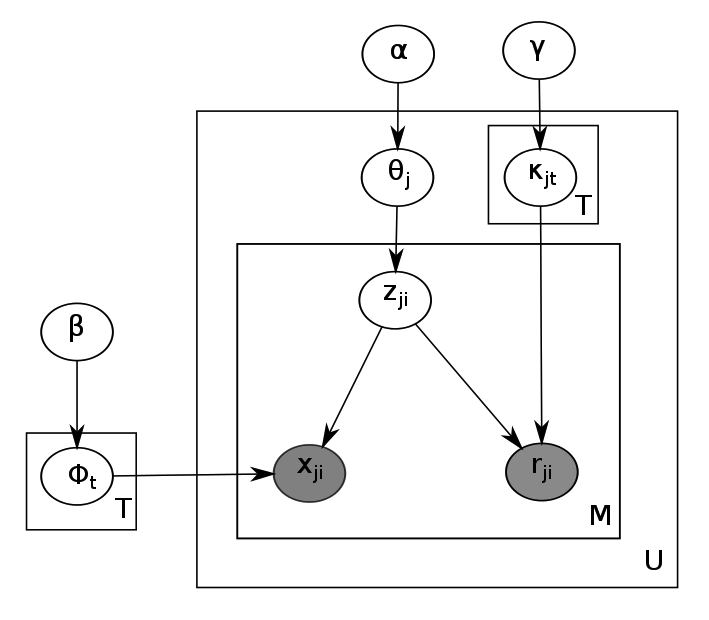
\includegraphics[width=.5\textwidth]{model.png}
      \caption{Representation of the Graphical Model}
      \label{fig:plot1}
    \end{center}
  \end{figure}
  
One can observe that this model resembles LDA, but with one change. We have 
included the rates, $r_{ij}$ that are given by a user to items, $x_{ij}$. We 
assume that each user has a different set of parameters, $\kappa_{tj}$, having a 
Dirichlet prior, which defines the rate with the topic assignment, $z_{ji}$. 
Note that rates are produced by a Categorical distribution with parameters, 
$\kappa_{jt}$. 

\section{Preliminary Experiment}
\label{exp}
In our preliminary experiment we will be analyzing the data in the MovieLens 100k
dataset \cite{movielens100k}. This dataset contains 100,000 ratings from 1,000
users on 1,700 movies. It is a well studied dataset for which we should be able
to obtain clean and comparable results. Our goal is to use LDA or a similar
algorithm to discover latent genres among the movies. As mentioned earlier,
since we will be using a generative model, we will also be able to generate
ratings for movies that users have not yet rated.

\cite{kermarrec:hal-00673330}

\section{Learning Algorithm}
\label{alg}
Before running any learning algorithm on a dataset with the above model, we 
should note that the matrix may contain incomplete data, meaning that not all 
users must rate every item out there. The classical algorithms don't deal with 
this issue. So, we will employ one or both of below approaches:
\begin{enumerate}
	\item First complete the matrix and then factorize it
	\item Run EM algorithm and operate on incomplete data likelihood as discussed 
	in \cite{Dempster77maximumlikelihood}
\end{enumerate}

After completing the matrix, we can use an MCMC algorithm to learn the hidden 
parameters of our model. Among this set of algorithms, we are going to use Gibbs 
sampler. However, if we find the mixing and convergence rate of the algorithm low, 
then we can employ variational methods which may be a better fit to large 
datasets. 

\section{Evaluation}
\label{eval}
Because we will be using a generative model we can partition our dataset into
training and testing parts. This will allow us to evaluate the reviews generated
for movie-user pairs in the test set. We can use widely adopted metrics such
as precision and recall to our model's effectiveness. In addition, because
the MovieLens dataset is widely used we will be able to compare our performance
against state of the art techniques.

Finally, to test the creation of the latent genres we can obtain expert defined
genres for a subset of the movies in the dataset. We can then use a metric to
analyze the distance between the predicted and expert defined genres.

\section{Timeline}
\label{time}

\begin{description}
	\item[11/16] Models and datasets finalized and any additional
			related work identified.
	\item[11/21] Initial results for MovieLens dataset collected.
	\item[11/25] Comparisons of results to existing baselines completed
			for initial results.
	\item[12/5] Finished collecting results for model(s).
	\item[12/7] Finished evaluation and comparison to existing models.
	\item[12/8] Project presentation completed.
	\item[12/13] First draft of paper completed.
	\item[12/16] Paper completed.
\end{description}
\bibliographystyle{plain}
\bibliography{main}

\end{document}
